
%(BEGIN_QUESTION)
% Copyright 2011, Tony R. Kuphaldt, released under the Creative Commons Attribution License (v 1.0)
% This means you may do almost anything with this work of mine, so long as you give me proper credit

This control valve acts as a crude proportional control system unto itself, used for controlling downstream pressure of a gas:

$$\includegraphics[width=15.5cm]{i01446x01.eps}$$

Suppose you are asked to increase the setpoint of this pressure-control system (so that the downstream pressure will now be regulated at a higher pressure).  How could you achieve this change, without replacing any of the valve's components or otherwise modifying the design of the pressure-control system?

\vskip 50pt

Suppose later on it was decided that the gas pressure control offered by this valve was too ``sloppy:'' the gas pressure drifts above and below setpoint too often and too far.  Explain how you could modify the system for increased {\it gain}, so that it will take more aggressive action to stabilize pressure.  Your re-design cannot add any new components to the system, but may modify the components already in place (e.g. replacing the control valve's packing with a different style).

\vskip 50pt

\underbar{file i01446}
%(END_QUESTION)





%(BEGIN_ANSWER)

Half-credit for each correct answer:

\vskip 10pt

To increase setpoint, one must {\it increase} spring tension so that more sensed pressure is necessary to return the valve to a condition of equilibrium.

\vskip 10pt

To increase gain, something must be changed to make the valve more sensitive to changes in sensed pressure.  One way to do this is increase diaphragm area.  Another way is to replace the spring with one having a lower (less stiff) constant.  Another way is to replace the valve trim with one having a greater $C_v$ rating, or one with a different characterization giving more aggressive gain in the region of most frequent use.

%(END_ANSWER)





%(BEGIN_NOTES)

{\bf This question is intended for exams only and not worksheets!}.

%(END_NOTES)


